\ylDisplay{Voltmeeter} % Ülesande nimi
{Tundmatu autor} % Autor
{lõppvoor} % Voor
{2015} % Aasta
{P 3} % Ülesande nr.
{3} % Raskustase
{
% Teema: Elektriõpetus

\ifStatement
 Kui suur on pinge, mida näitab voltmeeter (vt joonis)? Voltmeetri takistus on väga suur. Takistite takistused on vastavalt $R_1 = 15$ $\Omega$, $R_2 = 85$ $\Omega$, $R_3 = 25$ $\Omega$ ja $R_4 = 175$ $\Omega$. Pinge vooluallika klemmidel on $U = 20$ V.
\begin{center}
	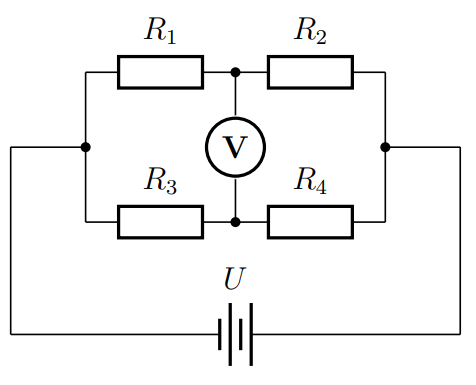
\includegraphics[width=0.5\linewidth]{2015-v3p-03-yl.png}
\end{center}
\fi

\ifHint
Voltmeetri näidu saab leides esimese ja kolmanda takisti pingete vahe.
\fi

\ifSolution
Harus, kus takistid $R_1$ ja $R_2$ on kogutakistus $R_u = R_1 + R_2$, mis on $100$ $\Omega$. Teises harus on kogutakistus $200$ $\Omega$. Esimeses harus on voolutugevus seose $I = I/R = 0,2$ A, teises harus $0,1$ A.
Pinge takistite $R_1$ ja $R_3$ otstes on seose $U = I R$ järgi $U_1 = 3$ V ja $U_3 = 2,5$ V. Seega on voltmeetri otstel pinge $0,5$ V.
\fi
}